% Chapter Template


\chapter{Einleitung: Zielstellung, Aufbau der Arbeit (1 Seite)}


Introduction layout:

- DMX etabliertes Protokoll mit vielen Lösungen.
Funktionieren aber auf der Anwendungsebene.

- Genaue Funktionsweise wird nicht erklärt, Nur übertragende Informationen angezeigt

-


\label{Chapter2} % Change X to a consecutive number; for referencing this chapter elsewhere, use \ref{ChapterX}

\lhead{Kapitel 2: \emph{Protokolle Lichttechnik}}

\chapter{Protokolle Lichttechnik: (8 Seiten)}

In der Lichttechnik haben sich mehrere Standards durchgesetzt. Abhängig vom Anwendungsfall werden meistens verschiedene Standards bevorzugt. Bei der Gebäudebeleuchtung wird DALI häufig genutzt. Aber auch neuere Technologien wie z.B. Zigbee oder Philips Hue setzten sich bei der privaten SmartHome Integration durch. In der Bühnentechnik hat sich der DMX Standard als industrieller Standard durchgesetzt. Der DMX Standard ist ebenfalls offen und kann von jedem implementiert werden. Allerdings sind die Leuchten, die auf dem freien Markt erhältlich sind, oft teuer.  Für die Signalsteuerung ist entweder ein DMX Controller oder DMX Software erforderlich. Auch diese sind oft teuer  oder lizenzpflichtig. In der Hobbyszene wird gerne ein anderes Protokoll dafür umfunktioniert: MIDI. Das Protokoll, wurde ursprünglich für die Übertragung von Musik erstellt, kann aber auch genutzt werden, um Lichtinformationen zu übertragen.


\section{DALI}
% TODO wie sieht das Datenpaket von DALI aus? - werden jedes mal alle Information gesenet, oder ist es nur eventbasiert?
Das Lichtsteuerungsprotokoll DALI (Digital Addressable Lighting Interface) ist in der Gebäudebeleuchtung weit verbreitet. Vor allem in Bürogebäuden, Hotels oder auch im Einzelhandel wird es oft verwendet. Einzelne Leuchten können spezifisch gesteuert oder zu Gruppen zusammengefasst werden.

DALI wurde erstmals in den späten 1990er \cite{DALI-2_certification} von der europäischen Lichtindustrie entworfen. Viele Hersteller verwenden seither das Protokoll weltweit für die Steuerung deren Produkte. Dadurch können Vorschaltgeräte von verschiedenen Hersteller nebeneinander eingesetzt werden, ohne dass der Anwender sich mit technischen Unterschieden auseinandersetzten muss \cite[p.2, ch. 3.1]{DALI-Lichtmanagement}.

Eines der Hauptvorteile von DALI ist die genaue Steuerung einzelner oder zu Gruppen zusammengefassten Leuchten. Jede Leuchte kann eine eindeutige Adresse zugewiesen werden. Die einzelnen Leuchten können dadurch separat voneinander gesteuert werden. Das Protokoll ermöglicht es, die Leuchten zu dimmen und somit maßgeschneidert an die speziellen Bedürfnisse der Umgebung anzupassen. Helles Arbeitslicht, Umgebungslicht als auch eine Akzentbeleuchtung kann damit gesteuert werden. Es können auch verschiedene Lichtszenen vorprogrammiert werden, z.B. eine Szene für die Tag- und Nachtbeleuchtung, (vgl.\ref{fig:dali_scenes}).

\begin{figure}[H]
	\centering
	\begin{subfigure}{.5\textwidth}
		\centering
		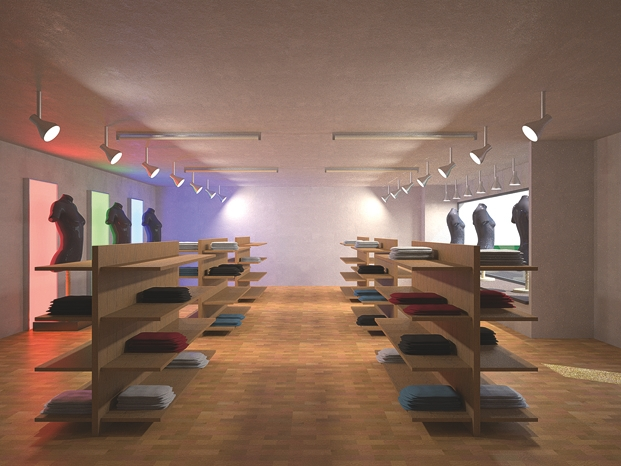
\includegraphics[width=.6\linewidth]{Pictures/DaliSchauraumTag}
		\caption{Szene Schauraum Tag}
	\end{subfigure}%
	\begin{subfigure}{.5\textwidth}
		\centering
		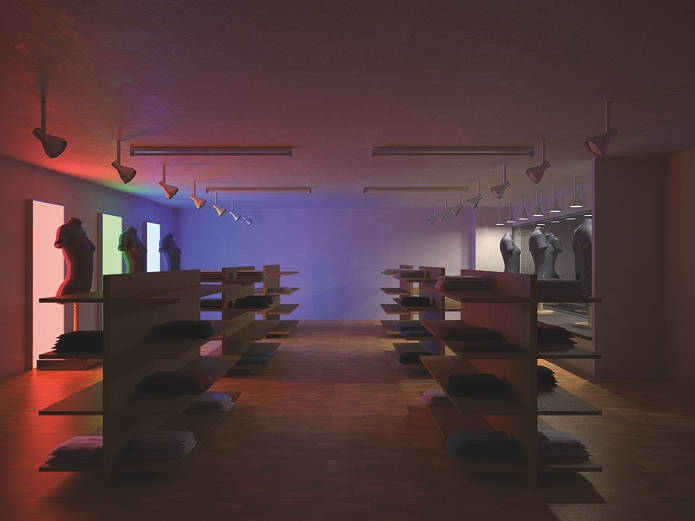
\includegraphics[width=.6\linewidth]{Pictures/DaliSchauraumNacht}
		\caption{Szene Schauraum Nacht}
	\end{subfigure}
	\caption{Beispiele für Lichtszenen \cite[p.6]{DALI_Handbuch}}
	\label{fig:dali_scenes}
\end{figure}

DALI ist ein digitales Protokoll, welches eine bidirektionale Kommunikation zwischen Leuchten und Controller ermöglicht. Dadurch können auch Fehlermeldungen der Leuchten ausgelesen werden. \cite[p. 1]{DALI-Lichtmanagement}. Eine kaputte Leuchte kann so einfach gefunden und ausgetauscht werden.  Aber auch andere Sensoren wie Tageslichtsensoren oder Bewegungssensoren können ins Netzwerk eingeschlossen werden. Damit kann die Helligkeit beispielsweise durch das Tageslicht oder durch die Anwesenheit von Menschen gesteuert werden. Der Stromverbrauch kann so massiv reduziert werden, da das Licht nur benutzt wird, wo es tatsächlich gebraucht ist.

DALI basiert auf einem einfachen zwei Kabel Bussystem. Das Bussystem kann am Ende des Busses fortgeführt werden, um es nachträglich zu erweitern. Der DALI Bus besteht aus zwei Leitungen. Ist die Verwendung von DALI gewünscht, so müssen ggf. diese Leitungen nachgerüstet werden. Wird dies bereits beim Bau eingeplant, können die freien Adern in einer Netzleitung benutzt werden\cite[p. c.3.2.2]{DALI-Lichtmanagement} (vgl.\ref{fig:wiring diagram}). Auf die Polarität der DALI Signale muss nicht geachtet werden \cite[p.3]{DALI_Handbuch}.

\begin{figure}[H]
	\centering
	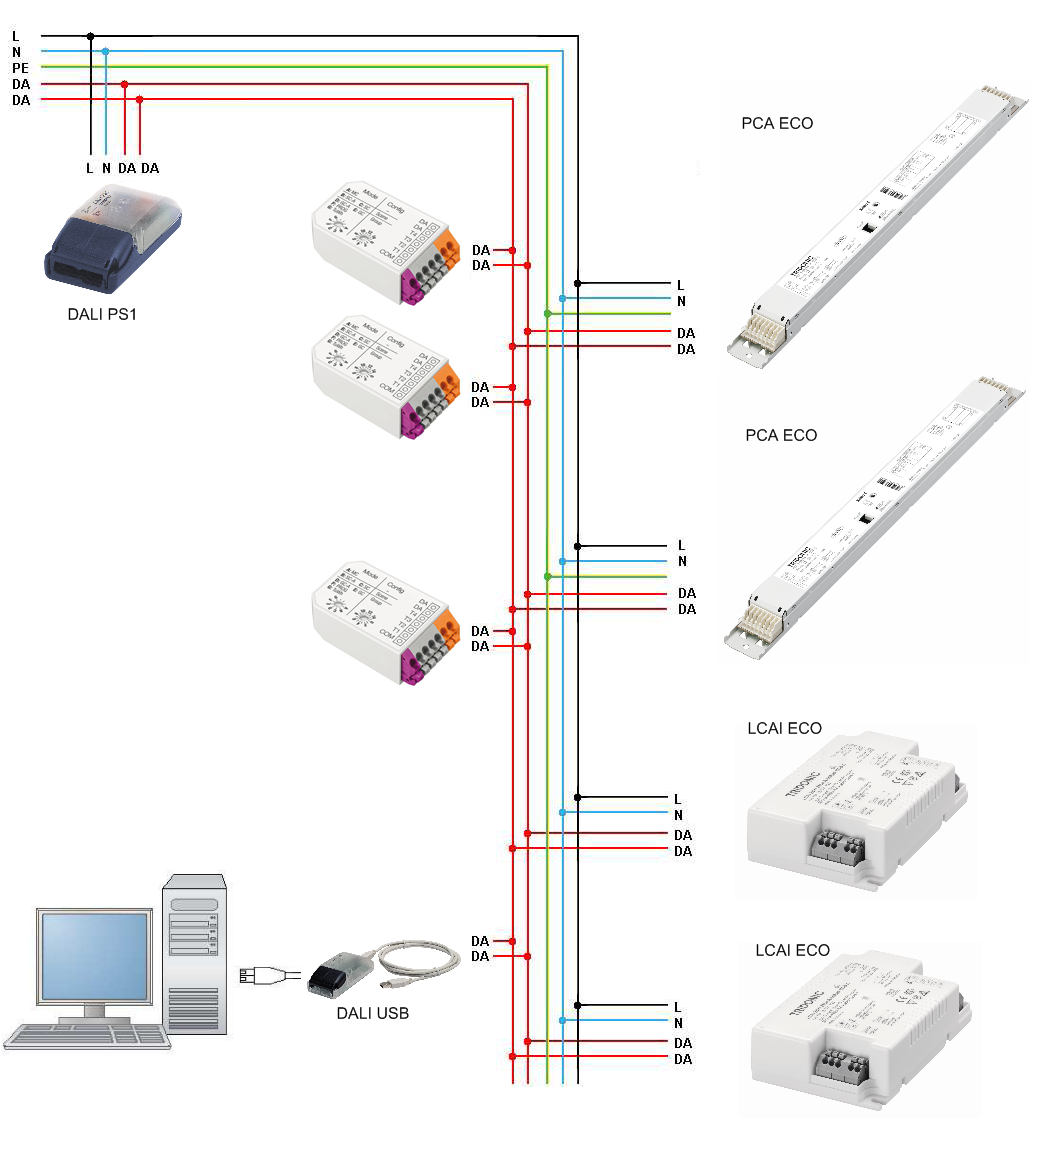
\includegraphics[width=.6\linewidth]{Pictures/DaliInstallation}
	\caption{Verdrahtungsdiagramm \cite[p.64]{DALI_Handbuch}}
	\label{fig:wiring diagram}
\end{figure}

Weiterhin können die DALI Controller einfach programmiert werden, um eine spätere Änderung der Leuchten einzustellen.

Neben den vielen Vorteilen hat das DALI Protokoll auch einige Limitierungen. Ein DALI Bus ist insgesamt auf max. 64 Adressen begrenzt \cite[p.7]{DALI_Handbuch}. Jede Adresse hat einen Wertebereich von 8 Bit \cite[p. 1]{DALI-Lichtmanagement}. Eine Leuchte kann daher z.B. auf max. 256 verschiedene Helligkeitsstufen eingestellt werden. Es können maximal 16 Gruppen und 16 verschiedene Lichtszenen programmiert werden. Die geringe Datenrate von 1200 Baud limitiert das Protokoll auf eine Aktualisierungsrate von ca. 25-30 Herz. Die Kabel können weiterhin maximal 300 Meter lang verlegt werden, bevor sie wieder verstärkt werden müssen \cite[p.3]{DALI_Handbuch}. 

Im Vergleich zu einem analogen System, hat DALI keine großen Probleme mit Interferenzen oder Störungen von externen Quellen. Das Protokoll ist selbst auf langen Strecken sehr zuverlässig.

Insgesamt ist DALI ein leistungsstarkes Lichtsteuerprotokoll, das durch seine Flexibilität, Genauigkeit und Energieeffizienz viele Vorteile gegenüber einem analogen traditionellen Steuersystem bietet. Die Adaption der Lichtindustrie hat es zu einem Industriestandard für die Gebäudebeleuchtung aller Art gemacht.

\section{DMX}

DMX (Digital Multiplex) ist ebenfalls wie DALI ein Lichtsteuerprotokoll. Der Anwendungsfall ist meist jedoch ein anderer. DMX ist der Industriestandard in der Bühnentechnik und Unterhaltungsindustrie. DMX wird benutzt, um steuerbare Leuchten zu koordinieren, wie z.B. bewegbare Leuchten und LED Leuchten. Dabei können alle Leuchten zentral von einem dedizierten physischen Controller oder via Software gesteuert werden.

DMX wurde erstmals im Jahr 1986 vorgestellt \cite[p.5, ch. 2.1]{DMX101-Handbook}. Seither wurde es der verbreitetste Industriestandard für koordinierte Lichtshows. Genau wie DALI, ist DMX ebenfalls ein digitales Steuerprotokoll. Über ein DMX Kabel kann jeweils ein DMX Universum übertragen werden. Ein DMX Universium kann mehere Känale gleichzeitig stuern. Ein Kanal kann dabei, z.B. auf die Rotation einer Leuchte, oder die Helligkeit einer Leuchte gemappt werden. DMX benutzt für die Übertragung eine serielle Übertragung basierend auf dem RS-485 Protokoll\cite[p.11, ch. 3.2]{DMX101-Handbook}.

Eines der Hauptvorteile von DMX ist die zentrale Steuerung von einer großen Anzahl von Leuchten über eine Konsole. Komplexere Leuchtkonstellationen mit vielen unterschiedlichen Leuchten sind dadurch umsetzbar. Mehrere Leuchten können so zusammengeschaltet werden, um komplizierte Effekte und Lichtszenen aufzubauen. Oftmals werden verschiedene Animationsmuster vorprogrammiert und als Preset eingespeichert. Lichtgestalter können dadurch einfach und schnell verschiedene Animationen und Konfigurationen aufrufen für die verschiedenen Phasen der Show.

Die Verkabelung von DMX ist einfach. In der Regel wird das Datensignal getrennt von der Stromversorgung geführt. Das Datensignal kann mithilfe einer Daisy Chain, (vgl. \ref{fig:dmx_wiring diagram}) einfach von Leuchte zu Leuchte weiter verbreitet werden. Am Ende der Daisy Chain, ist ein Terminator erforderlich, um die Datenintegrität innerhalb des Busses zu gewährleisten. Bei größeren Distanzen (ab 300 Meter) muss das DMX Signal geboosted werden, um eine sichere Datenübertragung zu gewährleisten.

\begin{figure}[H]
	\centering
	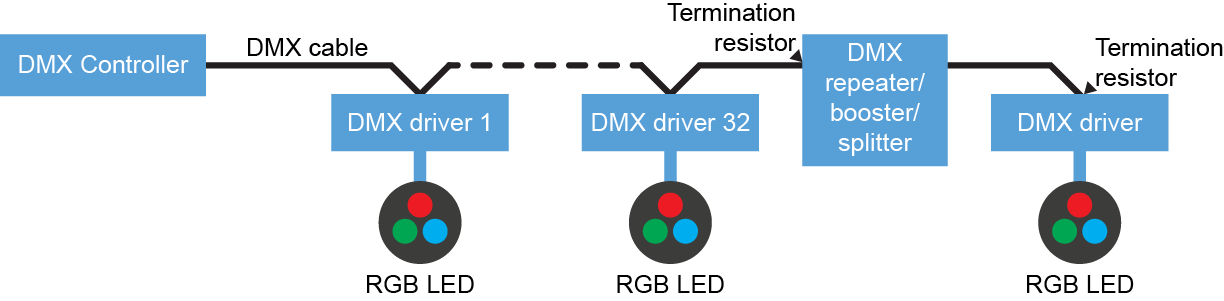
\includegraphics[width=.9\linewidth]{Pictures/dmxWiringDiagram}
	\caption{Verdrahtungsdiagramm \cite[p.64]{DMX_Wiring}}
	\label{fig:dmx_wiring diagram}
\end{figure}

DMX ist unter anderem auch sehr flexibel und konfigurierbar. Das Protokoll erlaubt die Ansteuerung von selbstgebauten Leuchten. Hersteller können für ihre Produkte auch bereits vorgefertigte DMX Presets mitliefern. Lichtgestalter bekommen dadurch eine genaue Kontrolle über die Funktionalitäten der einzelenden Leuchten. Wie z.B. die Farbeinstellungen oder Filter Auswahl.

Ein weiterer Vorteil von DMX, ist die Möglichkeit mehrere Systeme zusammenzuschalten. Eine große Anzahl an DMX Universen können über eine Konsole gesteuert werden, um eine größere Anzahl an Leuchten zu steuern. DMX kann auch mit Audio oder Video Systemen integriert werden, um eine synchrone Licht und Sound Show mit visuellen Effekten aufzubauen.

Neben den vielen Vorteilen, hat DMX auch einige Einschränkungen. Ein ungeboostest Signal kann maximal 300 Meter laufen, bevor das Signal durch durch die Signalverschlechterung erneut geboostet werden muss. Daher müssen für längere Strecken zwingend DMX Repeater verwendet werden, um die Signalstärke beizubehalten. Ein DMX Universum erlaubt eine Kontrolle von bis zu 512 Kanälen. Die Datenpackete werden mit einer Datenrate von insgesamt 250 kbps gesendet. Sind alle Kanäle ausgeschöft, ist die maximale refresh rate 44 updates/s \cite[p. 18, table6]{DMX512-Protocol-Standard}

Zusammengefasst ist DMX ein mächtiges Lichtsteuerungs-Protokoll, welches in der Industrie überall zu finden ist. Die Möglichkeit mehrere Leuchten getrennt voneinander ansteuern zu können, und die Integrierbarkeit mit anderen Systemen, hat es eine wesentliche Komponente für Lichtgestalter gemacht.


\section{MIDI}
%TODO optional: maybe talk about a bit about midi 2.0

Das Protokoll MIDI (Musical Instrument Digital Interface) ist ein Musikprotokoll, welches die Art und Weise wie Musik aufgenommen und erschaffen wird revolutioniert hat. MIDI erlaubt es elektronische Musikinstrumente, Computer, oder auch andere Geräte wie z.B. Synthesizer, miteinander zu interagieren. Musiker können dadurch den Sound eines Instrumentes live anpassen, und neue Effekte auf kreative Art und Weise erstellen.

MIDI wurde zuerst in den frühen 1980er Jahren \cite[p.1]{MIDI-Complete-SPECIFICATION} vorgestellt, und hat sich schnell als neuer Standard für die elektronische Musik Produktion durchgesetzt. Das Protokoll erlaubt eine Übertragung von musikalischer Daten, wie Note-on, note-off, Tonhöhe, Dämpfung, Modulation usw. zwischen MIDI-Kompatiblen Geräten \cite[p. 9]{MIDI-DETAILED-SPECIFICATION}. Dadurch können Künstler Musik mit einem elektronischen Keyboard aufnehmen und auch die Töne, zusammen mit Metainformationen, wie dem Tastendruck, Dauer des Tastenanschlages usw. aufnehmen, und auf einem anderen Gerät abspielen oder auch im Nachhinein verändern. 

MIDI kann auch benutzt werden um virtuelle Instrumente zu simulieren und mit Software Plugins, diese klanglich stark zu verändern. Künstler haben dadurch eine viel zahl von verschieden Sounds und Effekten zur Auswahl.

Ein weiterer Pluspunkt von MIDI ist die große Anzahl von Geräten, die MIDI unterstützen. MIDI kompatible Geräte beinhalten elektronische Tasteninstrumente, Synthesizer, Drum-Maschine und viele weitere. Künstler können einfach eine Vielfalt von Geräten zusammen benutzen, und neue kreative und raffinierte musikalische Werke produzieren.

Im Vergleich zu DMX agiert das MIDI Protokoll etwas anders mit Nachrichten. DMX sendet jedes mal alle aktiven Kanäle. Sollte ein Paket nicht beim Empfänger ankommen, ist dies kein Problem, da das nächste Paket wieder alle Informationen enthält. Leider werden dadurch Informationen, die sich nicht ändern, jedes mal neu versendet. MIDI hat einen anderen Ansatz: Es werden nicht kontinuierlich alle Informationen gesendet. Events, wie z.B. note-on beim Tastenanschlag, werden einmal gesendet \cite[p. 3]{MIDI-DETAILED-SPECIFICATION}. Dadurch werden keine Informationen redundant versendet.

Das MIDI Protokoll wurde erweitert, um neben den Musikinformationen, zusätzlich auch Lichtinformationen versenden zu können \cite[p. 1]{MIDI-Visual-Control} (vgl.\ref{fig:Midi_Light_Integration}). Die Leuchten, können programmiert werden, um auf Note-on und Note-off events zu hören \cite[p. 4]{MIDI-Visual-Control}. Über Effect-Control Events können Farben und weitere Optionen eingestellt werden \cite[p. 6, ch. 2.2.1.2]{MIDI-Visual-Control}. 

\begin{figure}[H]
	\centering
	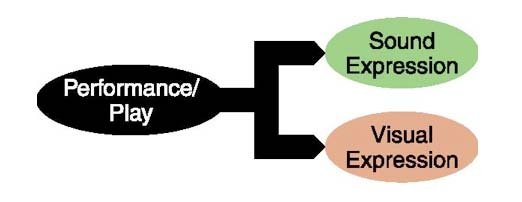
\includegraphics[width=.6\linewidth]{Pictures/MidiVisual}
	\caption{MIDI Licht Integration \cite[p. 1]{MIDI-Visual-Control}}
	\label{fig:Midi_Light_Integration}
\end{figure}


Neben den vielen Vorteilen, hat MIDI aber auch einige Einschränkungen. Gegen intuitiver Weise, ist MIDI nicht in der Lage, rohe Audiodateien zu versenden. MIDI kann nur digitale Signale verschicken, welche die Parameter und Benutzung der Musikinstrumente beschreibt. Daher ist auch ein separates Audio Signal erforderlich, um die Musik aufzunehmen, die mithilfe von MIDI erstellt worden ist. MIDI läuft mit ca. 31 kBaud. \cite[p. 1]{MIDI-DETAILED-SPECIFICATION}. DMX hat im Vergleich dazu eine 8 mal höhere Datenrate. 

Die genaue und flexible Einstellungen, hat es für Musiker eine wesentliche Komponente für die Musikproduktion gemacht.


\section{ZigBee}
% TODO optional: maybe include matter(application layer) (thread is physical layer)? its a IOT protocol
ZigBee ist ein Kabelloses-Protokoll, welches in den letzten Jahren stark an Popularität gewonnen hat. Es wird gerne für die Smart Home Automatisierung eingesetzt. Philips Hue ist ein Smart Home Produktgruppe, welches über ZigBee läuft, um Benutzer die Steuerung von Leuchten z.B. in einer Wohnung über das Smartphone zu ermöglichen. Auch eine Integration mit anderen Systemen ist möglich. So kann das Lichtbild an die Musik angepasst werden, oder Schalosien, am Abend automatisch heruntergefahren werden.

ZigBee und IEEE 802.15.4 sind standardisierte Protokolle, welche die Netzwerkinfrastruktur bereitstellen. Dabei definiert der IEEE 802.15.4 Standard den physikalische Layer, inklusive dem MAC Adressen. ZigBee definiert die Netzwerk- und Anwendungsschicht \cite[p.5]{GettingStartedWithZigBee}.

ZigBee hat einen geringen Stromverbrauch mit entsprechend verlangsamte Datenraten. Dadurch können auch batteriebetriebene Produkte lange durchhalten. Das Protokoll wurde entwickelt, um mit allen möglichen IoT (Internet of Things) Geräten zu kommunizieren.

ZigBee Geräte kommunizieren mit einer Mesh-Netzwerk-Topologie \cite[p.10]{GettingStartedWithZigBee}. Das bedeutet, jedes Gerät (oder auch jeder Knotenpunkt) kann als Repeater fungieren, um die Netzwerkreichweite zu vergrößern. Dadurch können ZigBee Geräte durch die Wohnung verteilt werden, um ein robustes und zuverlässiges System aufzubauen.

Philips Hue ist ein Produkt, welches sich auf smart LED Leuchten fokussiert. Es kann auch mit anderen ZigBee kompatiblen Geräten verschaltet werden. Philips Hue kann per App einfach übers Handy gesteuert werden. Die Helligkeit, Farbwärme oder auch ein Flackern wie bei einer Kerze kann eingestellt werden. Philips Hue kann unter anderem auch über Sprachassistent wie Alexa oder dem Google Assistenten gesteuert werden.

Ein weiterer Vorteil vom Hue System, ist der einfache Aufbau und Einrichtung. Mithilfe der Hue App können licht Szenen erstellt und abrufen werden. Timer können mit einprogrammiert werden, und mit einer Internetverbindung von überall (auch außer Hause) ferngesteuert werden. Auch können Bewegungsmelder, Dimmer oder Batterie betriebene smart Schalter benutzt werden, und überall im Hause verteilt werden, um die Lichter entspannt von überall aus steuern zu können. Auch smarte Steckdosen können mit dem System kontrolliert werden. 

Die Frequenzbänder von ZigBee überlappen sich mit den Frequenzbänder von Bluetooth und WLAN (vgl.\ref{fig:ZigBee_Frequency_bands}).
\begin{figure}[H]
	\centering
	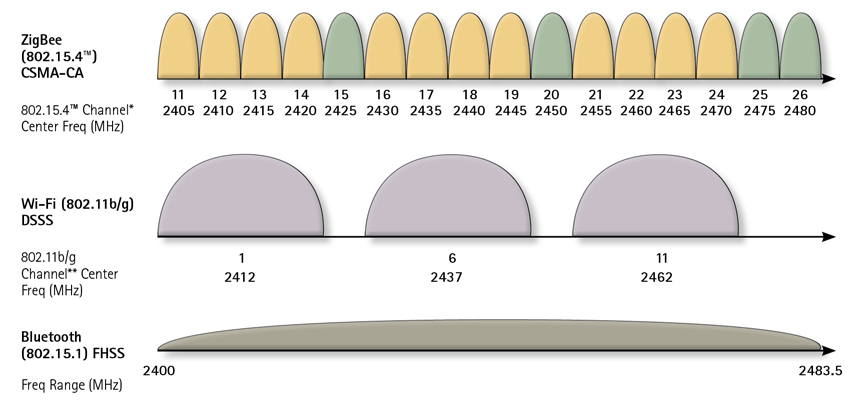
\includegraphics[width=.8\linewidth]{Pictures/ZigBeeRfOverlap}
	\caption{ZigBee Frequenzüberlappung \cite[p.23]{GettingStartedWithZigBee}}
	\label{fig:ZigBee_Frequency_bands}
\end{figure}
Die grauen Bänder haben weniger Überlappungen mit dem WLAN Kanälen. Sie können gewählt werden, um weniger Interferenzen zwischen den beiden Protokollen zu erhalten.

Durch die Kabellose Kommunikation ist keine Nachrüstung erforderlich. Dies erleichtert den Einstieg für Konsumenten erheblich. Sie müssen keine neuen Kabel verlegen, oder sich mit der Elektronik auskennen. ZigBee ist ein allgemeines Protokoll welches für IoT Geräte aller Art entwickelt worden ist. Es wird aber auch gerne bei Lichtinstallationen in privaten Wohnungen oft wieder gefunden.

Zusammengefasst hat das ZigBee Protokoll und die Philipps Hue Produkte eine neue Nische im Smarthome gefunden. Vor allem die einfache Installation und Nachrüstung macht es für den Verbraucher sehr einfach, auf Philips Hue umzuwechseln.


%TODO Tabelle / Grapfik zum Vergleichen der verschiedenen Protokolle




\chapter{Technischer Hintergrund (5 Seiten)}
\section{DMX}

\begin{figure}[H]
	\centering
	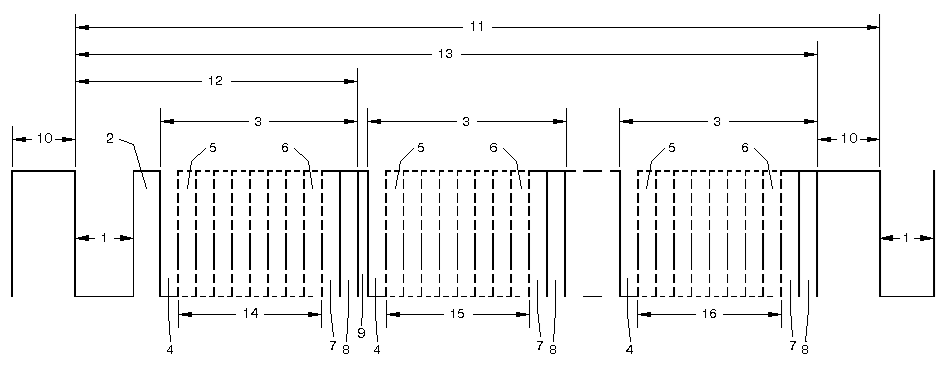
\includegraphics[width=\linewidth]{Pictures/DmxTimingFrame}
	\caption{Zeitdiagramm \cite[p.17]{DMX512-Protocol-Standard}}
	\label{fig:DmxTimingFrame}
\end{figure}

DMX Platine: Vorbild

\begin{figure}[H]
	\centering
	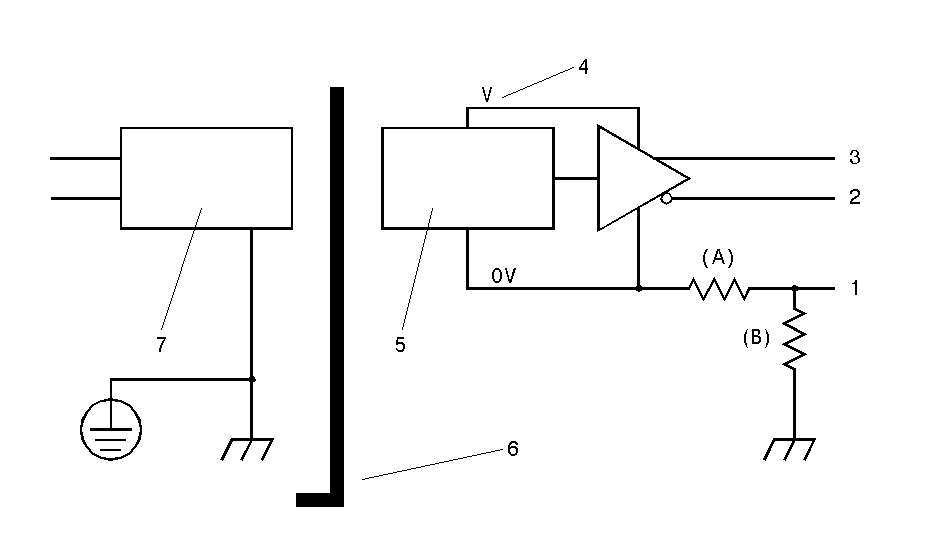
\includegraphics[width=0.5\linewidth]{Pictures/DmxIsolation}
	\caption{Zeitdiagramm \cite[p.22]{DMX512-Protocol-Standard}}
	\label{fig:DmxIsolation}
\end{figure}


\section{LED Matrix}
\section{SPI}
\section{OLA}
\section{UART}

\chapter{Implementierung (15 Seiten)}
\section{RPI Setup}
\section{OLA Setup}
\section{Coding environment setup (install dependencies)}
\section{Gehäuse Aufbau}

\chapter{Validierung: Studie (10 Seiten)}
\section{Aufbau}
\section{Durchführung}
\section{Ergebnis}

\chapter{Fazit (2 Seiten)}
